\documentclass[conference]{IEEEtran}
\IEEEoverridecommandlockouts
% The preceding line is only needed to identify funding in the first footnote. If that is unneeded, please comment it out.
\usepackage{cite}
\usepackage{amsmath,amssymb,amsfonts}
\usepackage{algorithmic}
\usepackage{graphicx}
\usepackage{textcomp}
\usepackage{xcolor}
\def\BibTeX{{\rm B\kern-.05em{\sc i\kern-.025em b}\kern-.08em
    T\kern-.1667em\lower.7ex\hbox{E}\kern-.125emX}}
\begin{document}

\title{Logistic Regression\\
%{\footnotesize \textsuperscript{*}Note: Sub-titles are not captured in Xplore and
%should not be used}
%\thanks{Identify applicable funding agency here. If none, delete this.}
}

\author{\IEEEauthorblockN{Pena Benafa}
\IEEEauthorblockA{\textit{Electronic Engineering} \\
\textit{University of Applied Science Hamm-Lippstadt}\\
Lippstadt, Germany \\
pena.benafa@stud.hshl.de}
}

\maketitle

\begin{abstract}
This seminar paper is an overview of logistic regression, one of the most used tools for predicting categorical outcomes. 
It uses a type of curve to fit data, and it describes the data and relationship between dependent variables and independent variables \cite{ab2}.
The main advantage of logistic regression is that it can predict the associated probability (this can be seen from the example given in this paper).
\end{abstract}

\begin{IEEEkeywords}
logistic regression, predicting, dependent variables, independent variables, data
\end{IEEEkeywords}

\section{Introduction}
The pioneer of machine learning (ML) defined ML as a "field of study that gives the computer the ability to learn without being explicitly programmed"\cite{bb1}. Thus, ML is a subset of Artificial Intelligence with roots in computational statistics, focusing on using computers to make predictions. Like humans that learn from experiences, the objective in ML is to create mathematical models that will train to make useful outputs (predictions) when fed with input or training data experiences). From these experiences, the ML models are tuned by an optimization
algorithm to produce accurate predictions. In addition, the ML models can generalize what they have learned from the training data (previous experience) so that they can make accurate predictions for new and unseen data\cite{bb2}.
An in-depth explanation and all the techniques in determining logistic regression percentage accuracy are discussed in section 2. Finally, section 3 concludes this seminar paper. 

\subsection{Types of Machine Learning Algorithms}
Different types of ML algorithms exist and are used to solve a variety of problems. ML algorithms can be grouped into three types of problems being solved: supervised learning, unsupervised learning, and reinforcement learning.

\subsubsection{Supervised Learning}
Consider the equation of straight line (Eq 1), in ML studies commonly referred to as regression equation.
               
\begin{equation} 
\label{equ1}
y = mx+b 
\end{equation} 

Where :\\
y = dependent variable \\
m = slope of the regression equation\\
x = independent variable\\
b = constant of the equation

In supervised learning, the ML model is given training data containing y and x. The model learns the relationship between these, i.e., m and b. Afterwards, the model is given test data with the only y; from its experience discovering m and b, it can predict the y's for each x. The classification of skin lesions according to malignancy is an example of this\cite{bb3}. Based on the value of the predicted label or dependent variable, supervised learning algorithms are further grouped into two, regression and classification. And logistic regression algorithm is an example of a classification supervised ML algorithm.\\

\subsubsection{Unsupervised Learning}
Unlike supervised learning, in which the training dataset of the ML model contains both the independent variables and dependent variable(s), in unsupervised learning, the training dataset contains only independent variables — x's. The ML model learns the relationship between all the independent variables and then groups them accordingly. An example of this is identifying and grouping customers who are high profit, high value or low-risk buyers\cite{bb4}. Unsupervised ML algorithms are grouped into the following: association, clustering and dimension reduction.

\subsubsection{Reinforcement learning}
Reinforcement learning is different from supervised and unsupervised learning. The problem dataset will contain at least independent variable(s); instead of reinforcement learning, an agent and an environment are constructed. Through trial and error, the agent learns from its environment while optimizing some set objective function. After every performed action, depending on the set goal, the agent gets a reward, punishment, or nothing. The agent uses these to determine the optimal path to the goal. The AlphaGo and AlphaZero are good examples of this \cite{bb3}, and \cite{bb5}.

\subsection{Description of the Classification Problem}
One of the problems in supervised learning is the classification problem. In this type of problem, the ML model built using ML classification algorithms learns from training datasets containing features or independent variables, i.e. x's, dependent variables or labels or classes (as they referred to in this case), i.e. y's. After training, the test dataset containing only the features are 'classified' or grouped according to what the model has learned from the training dataset. The classes can be binary, true or false, spam or not spam, 0 or 1, dog or cat, male or female e.t.c. Or the dependent variables can be multi-class; that is, instead of being 0 or 1, spam or not, there can be third, fourth….nth class. For example, classification of Apps in the App Store, an App can be classified as one of these, social media, game, news, weather, media (audio, photo, video), educational, health and fitness, entertainment e.t.c. In this seminar paper, the focus shall be on binary classification problems.


Here are some examples of ML algorithms used for solving classification problems:
\begin{enumerate}
\item Logistic Regression
\item Support Vector Machine
\item k-Nearest Neighbours
\item Decision Trees
\item Naive Bayes
\item Random Forest etc.
\end{enumerate}

\section{Logistic Regression}
Logistic regression can estimates probabilities using a logistic function to measure the relationship between independent variables and categorical (binary or multi-class) dependent variables. During the training phase, the ML model learns the relationship between categorical dependent variables and the independent variable(s). Then, in the test phase, for a given x, the model makes a prediction based on the probability that the corresponding y value for that x is "false" or "true". The sum of the
probability for these two outcomes is 1. However, the 'y' value would be "false" if the probability value for "false" is greater than "true". As mentioned earlier, the probability of the outcome is governed by a logistic function.

\subsection{Logistic Function}
Visually the shape of the logistic curve is shaped like an "S", and it is also called a sigmoid curve.
A sigmoid curve that shows a sufficient degree of smoothness is a bounded differentiable real function defined for all the real input values that have a positive derivative\cite{bb7}. The curve starts low, has a period of acceleration, and then approaches a straight line that defines the limit of a curve (asymptote).

\begin{figure}[h]
    \centering
    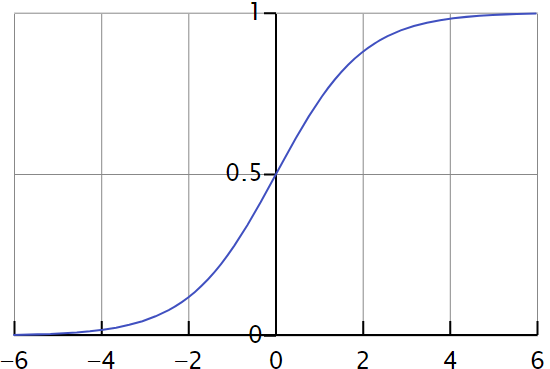
\includegraphics[scale=0.62]{figs/Lfunction.png}
    \caption{Graph of the standard logistic sigmoid function \cite{img}}
    \label{dabc}        
\end{figure}

\begin{equation} 
\label{equ2}
f(x) = \frac{L}{1 + e{^{-k(x-x0)}}}
\end{equation} 

Where:\\
L = the curves maximum value or the carrying capacity\\
k = the curves steepness or logistic growth rate\\
x = the independent variable\\
x0 = value of x at sigmoid's midpoint\\

The maximum value of f(x) is obtained when it approaches L, that is when x approaches $+\infty$. And the minimum value of f(x) is obtained when it approaches zero, that is when x approaches $-\infty$.

\subsection{Making Predictions (Example on Binary Logistic Regression)}
The dataset used for this coding example, is simple social network advert datasets, that contains 5 columns: UserID, Gender, Age, Estimated Salary and Purchase.\\
\\
UserID —: the social network's user's ID\\
Gender —: gender of the user\\
Age —: age of the user\\
Estimated-Salary —: estimated salary of the user and\\
Purchase —: purchase information about the user whether he/she purchased the advertised product through the social network.

\begin{figure}[h]
    \centering
    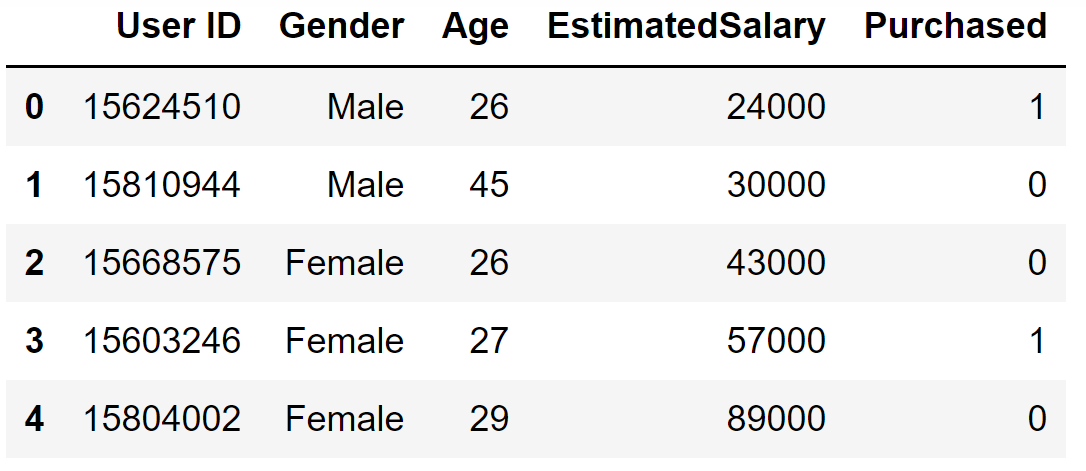
\includegraphics[scale=0.34]{figs/socialDataset.png}
    \caption{First five rows of the social network ad dataset}
    \label{dabc}        
\end{figure}


\subsubsection{Independent Variables (x)}
The independent variable shown in the fig 2, are the Age and Estimated Salary. These variables do not depend on other variables.

\subsubsection{Dependent Variables (y)}
The y variable is completely depended on x variables and from fig 2 above, the purchased column is the dependent variable, as it has two classes 0 and 1.\\
\\
Where :\\
1 —: indicates that the user purchased the the advertised product through the social network.\\
0 —: indicates that the user DID NOT purchase the the advertised product through the social network.\\

\subsubsection{Data manipulation}
The independent variables and dependent variables were separated from the main dataset, X and y, respectively.
After that, X and y were randomly split into a training set and test set. The training set had 75\% of the total dataset, while the test set had 25\%. Thus, both the training set and test set had X and the corresponding y values.
The training set was used to train the ML model, while the test set was used to evaluate the model, to check how good or bad it was.\\
Furthermore, independent variables for both the training and set were feature scaled. This was done to bring the variables to the same scale. Since the maximum value for Age is less than 100, the maximum value for the EstimatedSalary is more than 200,000. Using these values might skew the results and thus produced a skewed and/or biased ML model. The standardised value for a sample of x can be calculated by using this equation.

\begin{equation} 
\label{equ3}
z = \frac{(x-u)}{s}
\end{equation} 

Where :\\
z = standardised value for x\\
u = the mean of the training samples\\
s = standard deviation of the training samples\\
\\
The figures below show the Age and EstimatedSalary columns before feature scaling and after applying the formula (3) above, it shows the Age and EstimatedSalary columns after feature scaling.

\begin{figure}[h]
    \centering
    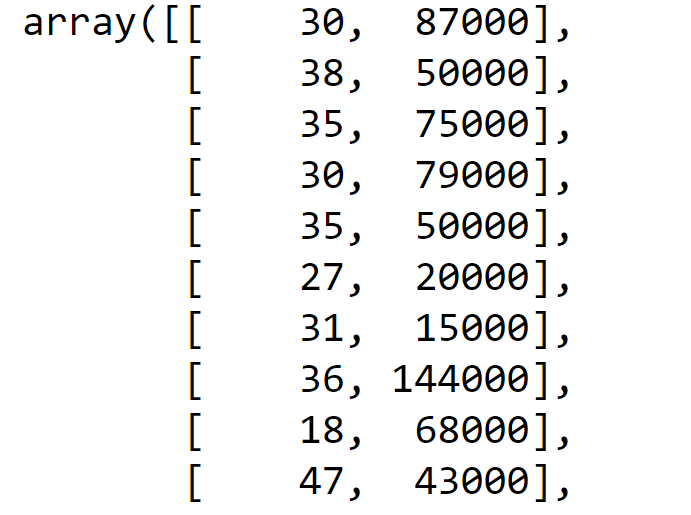
\includegraphics[scale=0.40]{figs/beforeFscaling.png}
    \caption{Age and EstimatedSalary columns before feature scaling}
    \label{dabc}        
\end{figure}

\begin{figure}[h]
    \centering
    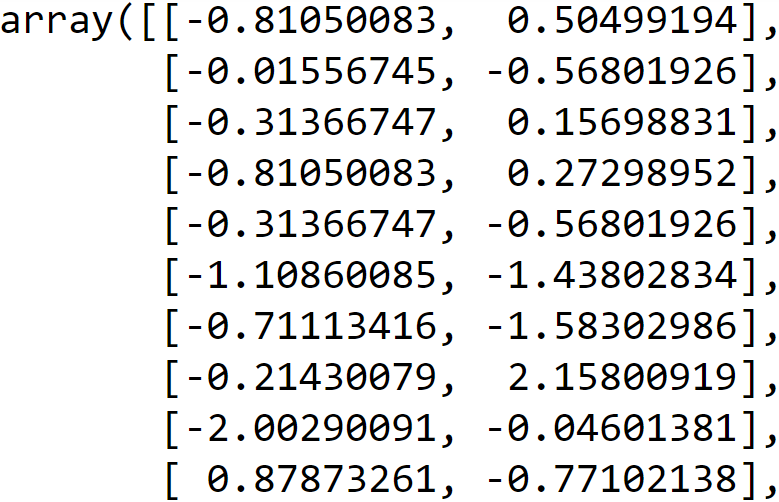
\includegraphics[scale=0.40]{figs/AfterFscaling.png}
    \caption{Age and EstimatedSalary columns after feature scaling}
    \label{dabc}        
\end{figure}


\subsubsection{Training}
After manipulation of the data, the training set was used to train the model. The figure below shows how the model classified the training dataset.

\begin{figure}[h]
    \centering
    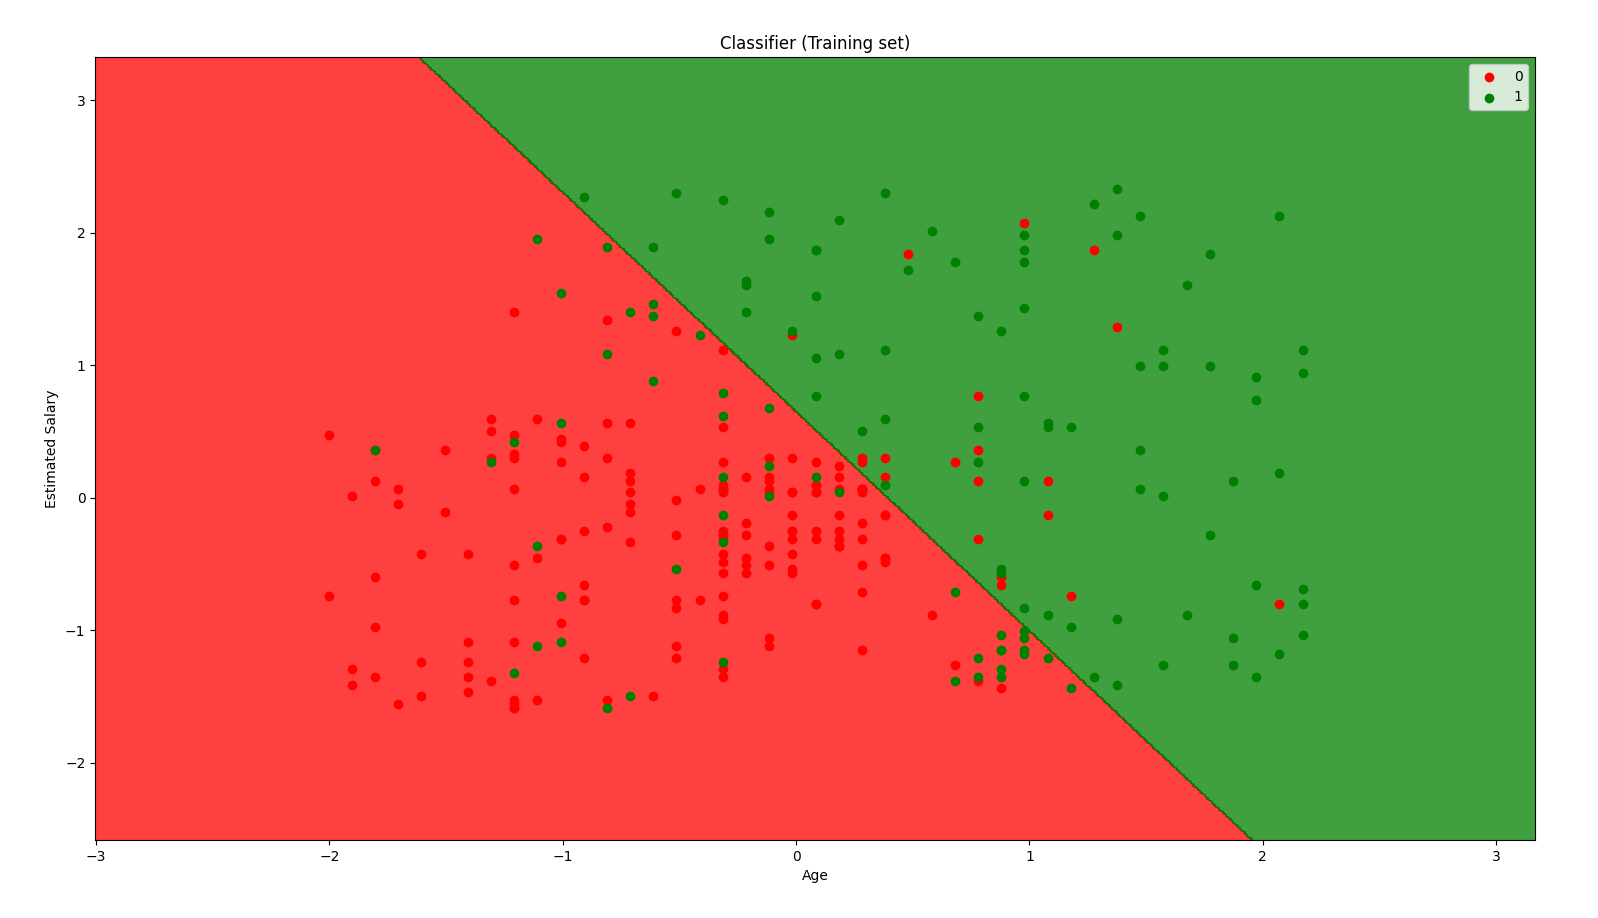
\includegraphics[scale=0.23]{figs/classTraining.png}
    \caption{Classification of the training set}
    \label{dabc}        
\end{figure}

\subsubsection{Evaluation Metrics}
Specific evaluation metrics are used to determine how good or bad a model is. For classification problems, the most common evaluation metrics are accuracy and confusion matrix. The accuracy is derivative of the four basic cardinalities of confusion matrix. Which are:\\
\\
1. True Positive (TP): predicted value is positive, and the actual value is positive, hence true.\\
2. True Negative (TN): predicted value is negative, and the actual value is negative, hence true.\\
3. False Positive (FP): predicted value is positive, but the actual value is negative, hence false.\\
4. False Negative (FN): predicted value is negative, but the actual value is positive, hence false.\\

\begin{figure}[h]
    \centering
    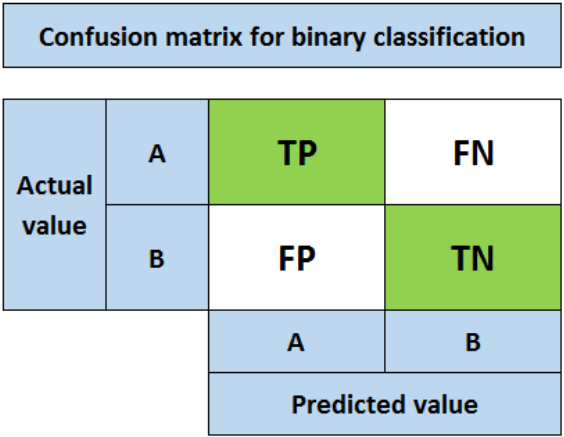
\includegraphics[scale=0.57]{figs/confusionMatrix.png}
    \caption{Confusion Matrix}
    \label{dabc}        
\end{figure}

\begin{equation} 
\label{equ4}
Accuracy = \frac{Totalnumberofcorrectpredictions}{Totalnumberofallprediction}
\end{equation}

\begin{equation} 
\label{equ5}
Accuracy = = \frac{TP + TN}{TP + TN + FP + FN}
\end{equation}
\\
For confusion matrix, the lower FN and FP, and higher TP and TN the better the model. The closer to 1.0, the accuracy is the better it is.\\

\subsubsection{Test set Prediction and Model Evaluation}
After training the model, the test set was predicted. As mentioned earlier, the test set contains both the independent variables and the dependent variable. Therefore, to know how good or bad the newly trained model was, the model was used to predict the test result. This means the independent variables were fed to the model, from which the model predicted the corresponding dependent variables.
After this, the predicted values of the dependent variables were compared with the actual values, using the evaluation metrics explained earlier. Fig (7) shows
how the model classified the test dataset.

\begin{figure}[h]
    \centering
    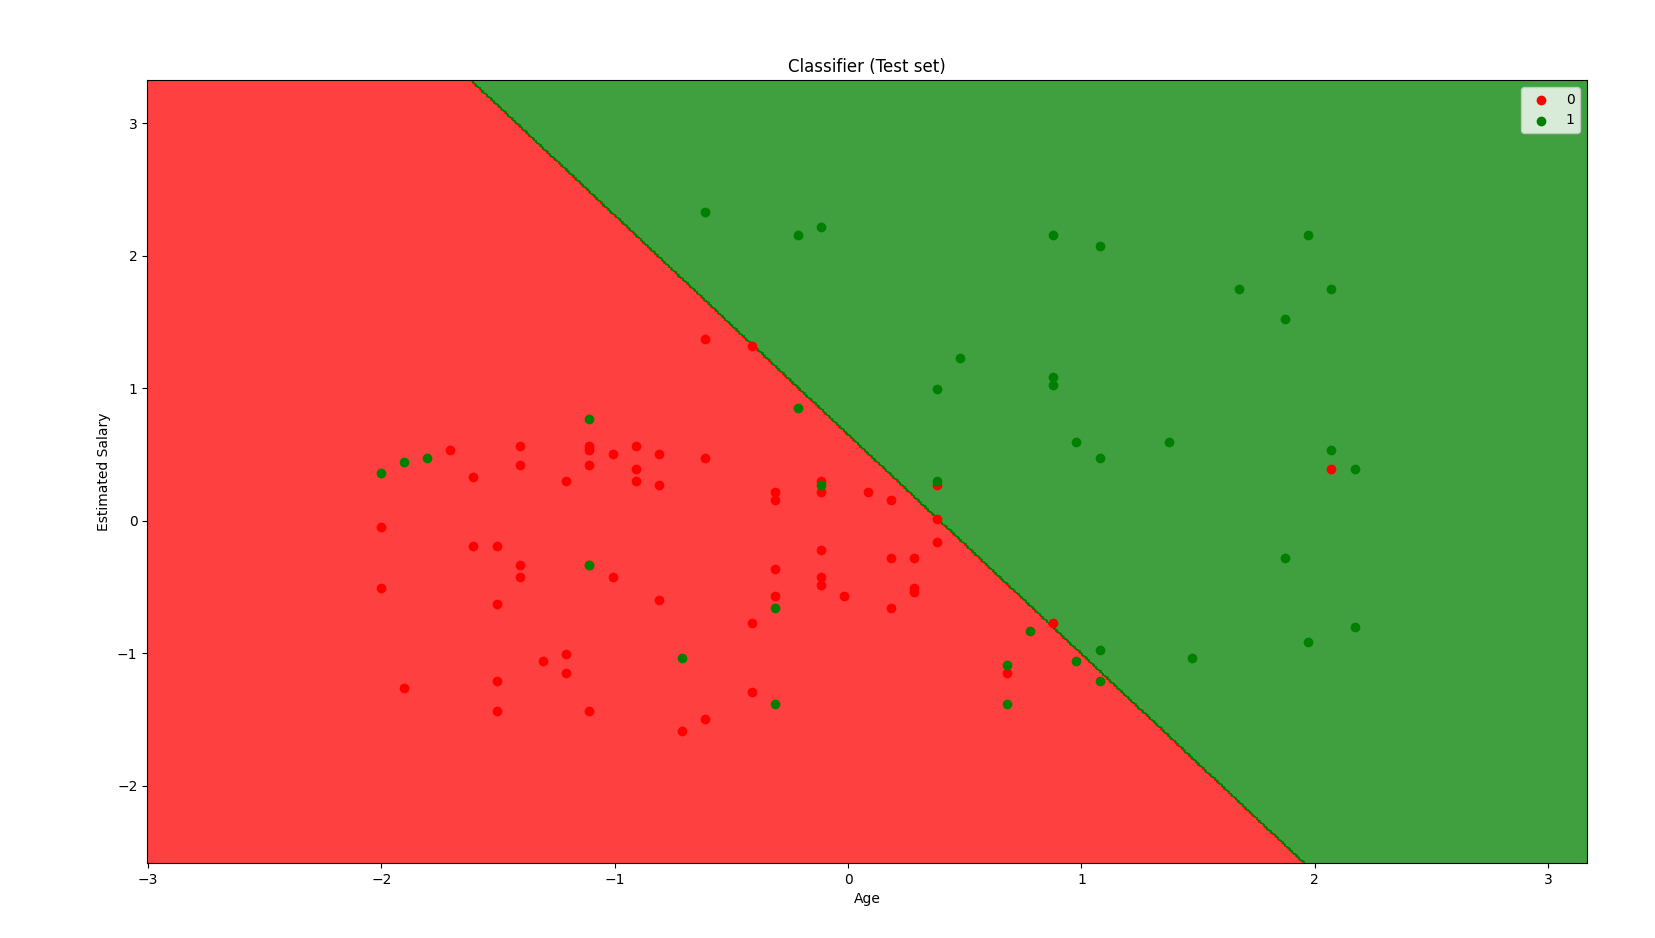
\includegraphics[scale=0.21]{figs/classTest.png}
    \caption{Classification of the test set}
    \label{dabc}        
\end{figure}

The accuracy for the test result was 0.82 which is very good. Using the confusion matrix, we can explain the accuracy when Logistic Regression Classification is applied to the supplied dataset.\\
The confusion matrix gives the following:\\
\begin{figure}[h]
    \centering
    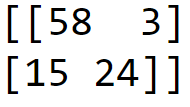
\includegraphics[scale=0.71]{figs/matrix.png}
    \caption{Confusion Matrix}
    \label{dabc}        
\end{figure}

This is entered in the diagram below and explained thus:\\
\\
1.	At the top left, it shows that the system correctly predicted 58 no purchase decisions.\\
2.	At the bottom right, the system correctly predicted 24 purchase decisions.\\
3.	At the top right, the system wrongly predicted 3 no purchase decisions as purchase decisions.\\
4.	At the bottom left, the system wrongly predicted 15 purchase decisions as no purchase decisions.

The confusion matrix gives the following:\\
\begin{figure}[h]
    \centering
    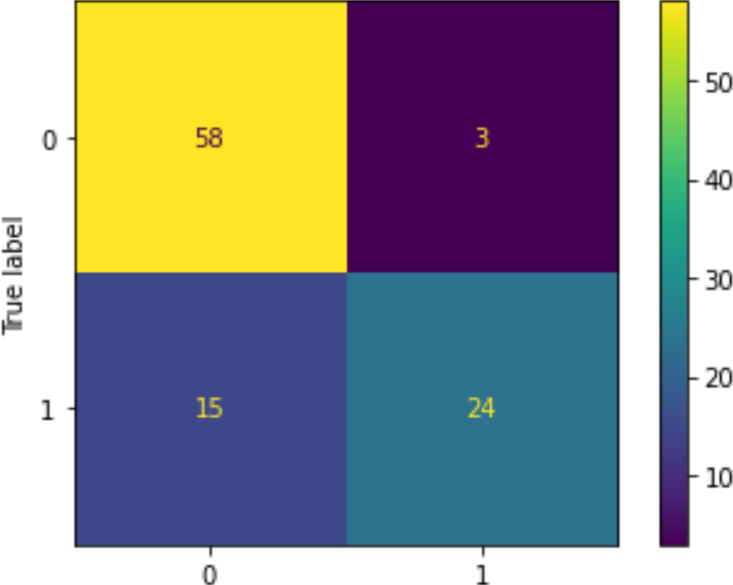
\includegraphics[scale=0.47]{figs/PredictL.png}
    \caption{Confusion Matrix Table for Logistic Regression}
    \label{dabc}        
\end{figure}


%\subsubsection{Decision Boundary}
%\section{Cost Function and Gradient Descent}
%\section{Over fitting Problem}
%\subsection{Under Fitting}
%\subsection{Over Fitting}


\section{Conclusion}
There are countless use cases of logistic regression and other classification machine learning algorithms across multiple industries and sectors. In the example,  the model I used could predict whether social network users will buy a particular product via network given their age and estimated salary. The example used is an oversimplified version of what is obtainable in a real social network like Instagram, Twitter or Facebook. In the real-life situation, there might not be an estimated salary; however, there would be a lot more independent variables that might include: race, employment histories, political interests, religion, sports interests and affiliations, time spent on the network per day, likes given to different posts, number of ads viewed, number of friends and family, and other information from friends and families e.t.c.\\
Although in the coding example, the obtained accuracy was 0.82, which is good. It might not be the best we can get for this dataset. Changing the training set and test set split ratio to 80/20 might improve the result or using another classification machine learning algorithms as kNN, SVC, Decision Trees, Random Forest e.t.c. It is known that no single algorithm is better than all the others on all the problems; however, certain algorithms stand up tall in certain problem\cite{bb6}. Thus, it is possible that logistic regression might not be the best for the problem in solved in the coding example.\\
\\
The code and dataset used for the coding example are available in:
https://github.com/Justblaise/Logistic-Regression

\section*{Acknowledgement}


%\section*{References}
\bibliographystyle{IEEEtran}
\bibliography{reference}


%\begin{thebibliography}{00}





%\end{thebibliography}

\end{document}
